\begin{thm}{024}{\hosi 6}{Jr. 算オリ Final}
 ひし形ABCDに$\mr{AE}=\mr{CF}$となる点を図のように取ります。図のようにア~エの4つの図形に分けると、アはウより155cm${}^2$小さく、イはエより31cm${}^2$小さいです。アの面積は何cm${}^2$ですか。
 \begin{center}
  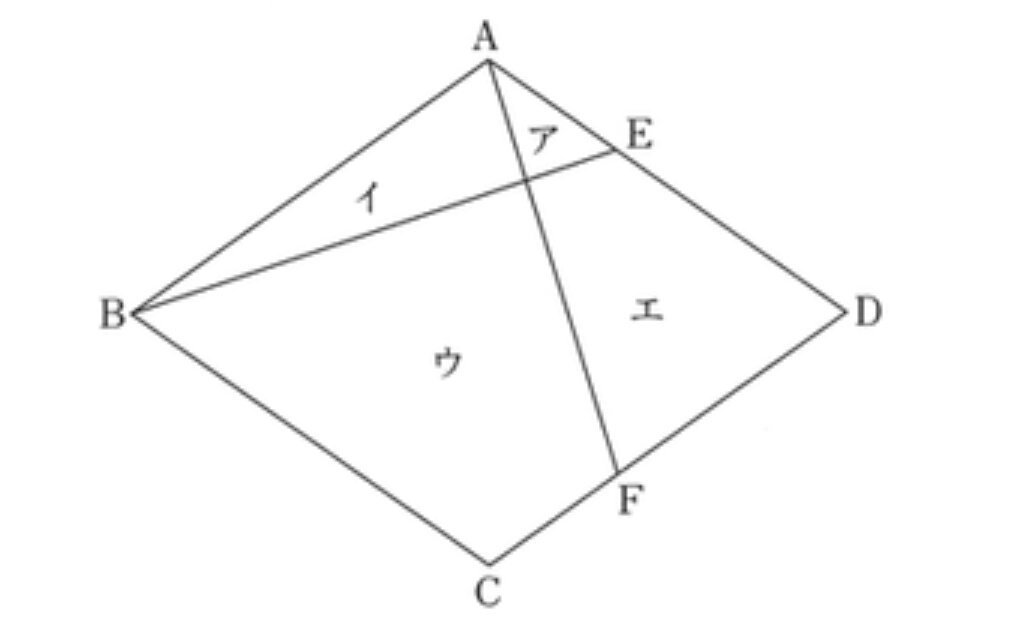
\includegraphics[bb=0 0 1013 637,width=0.7\linewidth]{../problems/Q_024/Q_024.jpg}
 \end{center}
\end{thm}

ここに解答を記述。